\documentclass[tcc,capa]{texufpel}
\usepackage[utf8]{inputenc} % acentuacao
\usepackage{graphicx} % para inserir figuras
\usepackage{verbatim}
\usepackage{hyperref}
\usepackage{float}
\usepackage{lipsum}
\usepackage{xcolor}
\usepackage{floatrow}
\usepackage{caption}
\definecolor{verde}{rgb}{0,0.5,0}
% Configurando layout para mostrar codigos C++
\usepackage{listings}
\lstset{
  language=C++,
  basicstyle=\ttfamily\small,
  keywordstyle=\color{blue},
  stringstyle=\color{verde},
  commentstyle=\color{red},
  extendedchars=true,
  showspaces=false,
  showstringspaces=false,
  numbers=left,
  numberstyle=\tiny,
  breaklines=true,
  backgroundcolor=\color{green!10},
  breakautoindent=true,
  captionpos=b,
  xleftmargin=0pt,
}
\pagestyle{empty}
\unidade{Centro de Desenvolvimento Tecnológico}
\curso{Engenharia de Computação}
\nomecurso{Bacharelado em Engenharia de Computação}
\titulocurso{Bacharel em Engenharia de Computação}
\title{Desenvolvimento de uma Solução para o Registro de Presenças e Controle de Acesso em Eventos Acadêmicos Utilizando Identificação e Comunicação por Radiofrequência}
\author{Silveira}{Rafael}
\advisor[Prof.~Dr.]{Marques}{Felipe de Souza}
\coadvisor[Prof.~Dr.]{Zatt}{Bruno}
\collaborator[Prof.~Dr.]{da Rosa Júnior}{Leomar}


\keyword{Automação}
\keyword{RFID}
\keyword{Zigbee}
\keyword{Sistema}

\begin{document}

%\renewcommand{\advisorname}{Orientadora}           %descomente caso tenhas orientadora
%\renewcommand{\coadvisorname}{Coorientadora}      %descomente caso tenhas coorientadora

\maketitle 

\sloppy

%\fichacatalografica
\begin{figure}
  \makebox[\textwidth][c]{\includegraphics{ficha}}
\end{figure}

%\folhadeaprovacao
 \begin{figure}[H]
            \centering 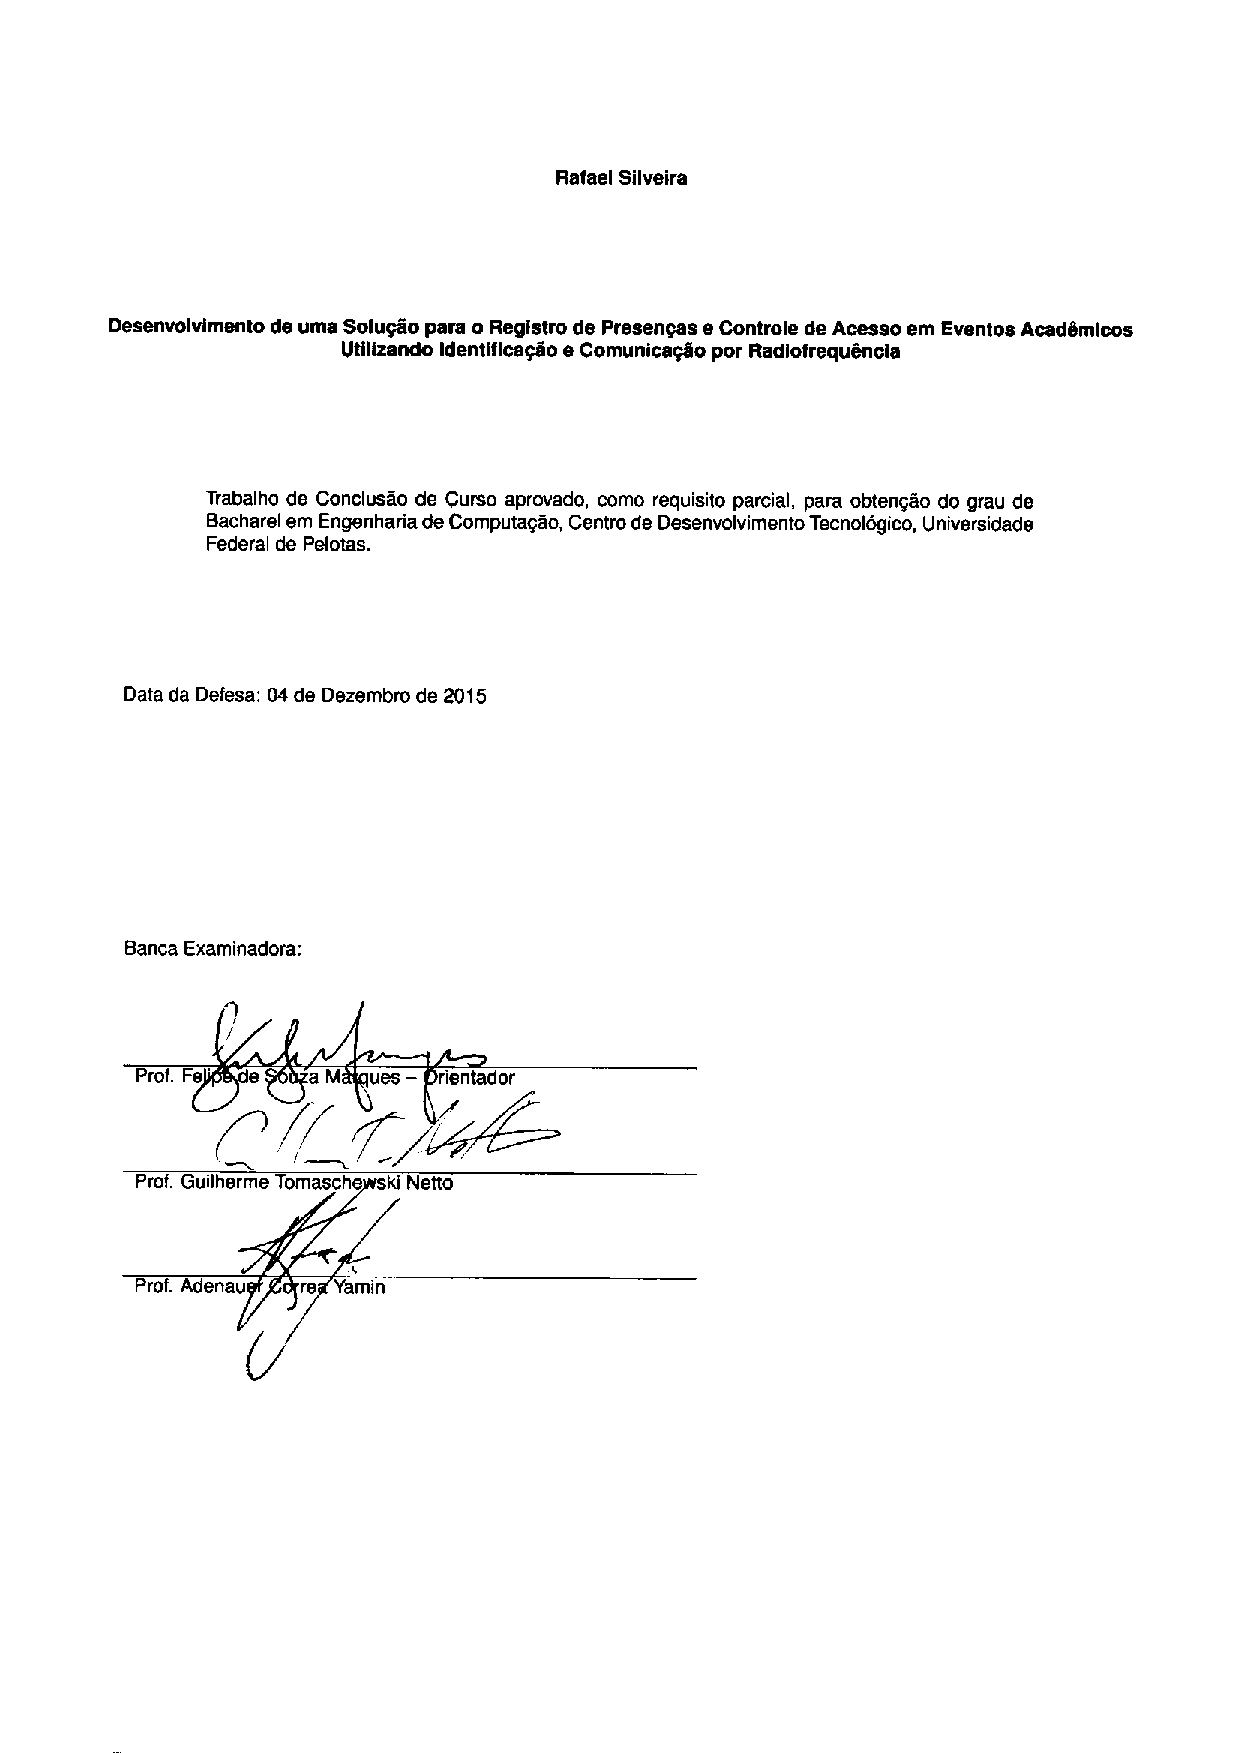
\includegraphics[scale=0.8]{folhaaprovacao}
            \label{folhaaprovacao}
        \end{figure}


%Opcional
\begin{dedicatoria}
  Dedico esta conquista ao meu querido avô Edy da Silveira.
\end{dedicatoria}

%Opcional
\begin{agradecimentos}
    Primeiramente, gostaria de agradecer a Deus, pois sem ele nada seria possível.
    Agradeço a toda a minha família e minha namorada, por compreenderem a minha ausência por conta da faculdade. 
    Agradeço também, aos professores Felipe Marques, Leomar Jr, Daniela Brauner e Bruno Zatt, por me ajudarem e incentivarem desde o inicio deste trabalho de conclusão.
    A todos os meus amigos e colegas integrantes do PET Computação, com certeza sem eles tudo seria tão chato e muito mais difícil.
    
    Por fim, e não menos importante, gostaria de agradecer todos os meus amigos de São Lourenço do Sul, que de uma forma ou outra, contribuíram para que eu pudesse chegar aqui.
\end{agradecimentos}

%Opcional
\begin{epigrafe}
Eu acredito demais na sorte. E tenho constatado que, quanto mais duro eu trabalho, mais sorte eu tenho.
\end{epigrafe}

%Resumo em Portugues (no maximo 500 palavras)

\begin{abstract}

Atualmente, não existe um sistema  para gerenciamento de eventos acadêmicos que integre eficientemente hardware/software. Eventos acadêmicos como congressos e semanas acadêmicas, cada vez mais vem tornando-se cansativos e inviáveis por conta de processos obsoletos de registro de presenças e controle de acesso.

Portanto, esse trabalho de conclusão de curso apresenta o desenvolvimento e validação de uma ferramenta automatizada para o registro de presenças e controle de acesso utilizando RFID (Identificação por Radiofrequência).
A solução proposta inclui o hardware necessário para fazer a leitura de etiquetas RFID, uma camada de middleware que implementa uma API para comunicação com o servidor de dados e, também, uma aplicação web com perfis para participantes e organizadores do evento.

O sistema foi validado e testado na XX Semana Acadêmica do Curso de Computação da Universidade Federal de Pelotas e acredita-se que os objetivos da proposta foram cumpridos, sanando os principais problemas apontados em edições anteriores do evento.

\end{abstract}

\begin{englishabstract}
  {Development of a Solution for the Record of Attendance and Access Control on Academic Events Using Identification and Communication by Radio Frequency}
 {Automation, RFID, Zigbee, System}
   Currently, there is no management system to manage academic events integrating hardware and software. Academic events, such as conferences and seminars, are hard to manage due to obsolete processes for attendance registration or access control.
Therefore, this work introduces the development and validation of a tool that automatizes the processes for attendance registration and access control using RFID tags.
The proposed solution includes the hardware needed to read RFID tags, a middleware layer that implements an API to access a data server, and a web application that may be used by attendants and organizers of the event.
The system was tested and validated during the 'XX Semana Acadêmica do Curso de Computação da Universidade Federal de Pelotas', and it have met the initial requirements, mitigating the main problems of past editions of the event.
\end{englishabstract}

%Lista de Figuras
\listoffigures

%Lista de Tabelas
\listoftables

%lista de abreviaturas e siglas
%\begin{listofabbrv}{SPMD}
 %       \item[RFID] Radio-Frequency IDentification
  %      \item[NUMA] Non-Uniform Memory Access
   %     \item[SIMD] Single Instruction Multiple Data
    %    \item[SPMD] Single Program Multiple Data
     %   \item[ABNT] Associação Brasileira de Normas Técnicas
%\end{listofabbrv}

%Sumario
\tableofcontents

\chapter{Introdução}
    "Casa de ferreiro, espeto de pau"~  é um ditado popular usado quando uma pessoa quer salientar que alguém se comporta de maneira diferente da que é incentivada pelo seu próprio discurso. Este ditado popular se aplica perfeitamente à situação que vive a Computação UFPel \cite{schmidt2011instituto}.
    
    É comum que, em eventos acadêmicos, a presença dos participantes seja registrada de alguma forma com a finalidade de controle e emissão de certificados. Normalmente, essa necessidade gera alguns inconvenientes como atrasos, perda do registro e até mesmo burlagem do sistema.
    
    Na Universidade Federal de Pelotas, mais precisamente na Computação, os registros de presenças em eventos são gerados utilizando-se um leitor de código de barras, o que, na Semana Acadêmica de 2014, causou filas, atrasos, reclamações e a necessidade de uma pessoa para realizar a tarefa. O que, posteriormente, resultou em um dos motivos da desistência de registro na edição do ano seguinte.
    
    No XXIII Congresso de Iniciação Científica (CIC) e XVI Encontro de Pós-Graduação (ENPOS), onde o controle foi feito via carimbo, houve a necessidade de um organizador por sala para o controle da presença e acesso, necessitando de, diversos organizadores especialmente selecionados para essa função. Além dos problemas salientados, atualmente soluções hardware/software não estão completamente difundidas em Pelotas e região, sendo que, as existentes, são extremamente caras.
    
    Visando solucionar esses problemas, este trabalho de conclusão de curso propõe uma solução de baixo custo, utilizando tecnologias inovadoras do mercado como: Identificação por radiofrequência (do inglês, \textit{Radio-Frequency IDentification} - RFID) e comunicação sem fio usando padrão ZigBee. Para processar essas informações, foi desenvolvido um sistema web com tecnologias atuais, tais como: PHP, HTML, CSS e banco de dados MySQL, o qual automatiza todo o processo desde a geração de boleto e processamento da presença ao desenvolvimento do certificado e envio ao participante via e-mail.

    
    \section{Motivação e Justificativa}
    	
    
         A tecnologia de RFID consiste em um termo genérico para as tecnologias que utilizam a frequência de rádio para captura de dados de identificação. Contudo, existem várias outras opções para identificação automática de pessoas e objetos, como é o caso dos códigos de barras, identificação biométrica, por voz e QR code.  A vantagem do RFID é permitir a identificação automática de pessoas e objetos, mas à distâncias consideráveis.
    
        Quanto aos métodos de identificação, o mais comum é armazenar um número que identifique uma pessoa ou um objeto, ou outra informação, em um microchip. Tal tecnologia permite a captura automática de dados, para identificação de objetos com dispositivos eletrônicos, conhecidos como etiquetas eletrônicas,\textit{tags} ou \textit{transponders}, que emitem sinais de radiofrequência para leitores que captam estas informações.
         
        
        O leitor RFID consiste em um módulo transmissor e receptor e unidade de controle. Muitos deles possuem interfaces adicionais como RS 232 e RS 485 para a comunicação com outros sistemas como computadores e servidores \cite{finkenzeller1999rfid}. Como essa comunicação é feita apenas com cabos, uma das justificativas deste trabalho é o desenvolvimento de uma solução sem fio com dispositivos utilizando o padrão Zigbee de comunicação.
        
        O padrão Zigbee é um protocolo de comunicação por radiofrequência de baixo consumo de energia \cite{faludi2010building}, o qual pode ser implementado por componentes eletrônicos denominados Xbee, Garabee, etc. Pode-se implementar diversas topologias como: árvore, malha e estrela. Dependendo do componente, pode ser feita uma comunicação de até 1500 metros de distância. Assim, torna-se possível a existência de diversos dispositivos leitores de cartões RFID distantes entre si, enviando seus dados para um servidor local que esteja conectado à internet.
        
        Outra justificativa, de acordo com \cite{Sundaram:2010}, os dois elementos cruciais das ciber-infraestruturas do futuro, são \textit{Web Services} e Identificação por radiofrequência. Existe uma necessidade de ligar esses elementos para desenvolver e-infraestruturas que permitam uma organização ser ágil e flexível . Além disso, especialistas em novidades da tecnologia afirmam que mais cedo ou mais tarde, dada a evolução do RFID, as etiquetas inteligentes estarão nos produtos que qualquer consumidor vier a comprar \cite{bernardo2004tecnologia}. 
        
        Porém, atualmente, não existe um sistema eficiente para gerenciamento de eventos que integre tanto hardware, quanto software na UFPel. Eventos acadêmicos como congressos e semanas acadêmicas, cada vez mais vem se tornando cansativos e inviáveis por conta de processos obsoletos de registro de presenças e controle de acesso. Problemas os quais poderão ser reduzidos com a automatização do processo com tecnologia RFID.
    
    
    
    %\section{Metodologia}
        
        %Este trabalho esta sendo desenvolvido seguindo uma metodologia incremental de leitura, escrita, codificação, prototipação e teste. Em primeiro momento, foi feito um estudo teórico sobre os microcontroladores da Atmel pertencentes a família AVR, leitores RFID e comunicação sem fio via módulos Zigbee. Em um segundo momento, após o hardware ter sido definido, foram realizadas simulações do sistema eletrônico em ferramentas de CAD a fim de prever possíveis problemas no projeto. Só então, foram adquiridos os componentes necessários e executados testes na protoboard.
        
        %Após completo domínio da área de hardware, iniciou-se o processo de modelagem sistema Web. Foi realizado o levantamento dos requisitos e modelagem usando Linguagem de Modelagem Unificada (do inglês \textit{Unified Modeling Language} - UML), a partir dos principais diagramas dessa metodologia, tais como: casos de uso e sequência. Também foi desenvolvida a modelagem conceitual do banco de dados e desenvolvimento de código utilizando metodologia incremental com auxílio de ferramenta de controle de versão.
        
        %Ao final do trabalho de projeto, desenvolvimento e seu processo de revisão, que foram desenvolvidos no TCC-1, pretende-se validar o sistema na Semana Acadêmica da Computação a partir do uso de crachás com tecnologia RFID em um grupo de participantes do evento.
        
        %Por fim, juntamente com o período que ocorreram as tarefas supracitadas, foi elaborada a monografia parcial e um resumo expandido para o Sulpet.
    
    \section{Soluções Existentes no Mercado}
    
        Existem diversas soluções para gerenciamento de eventos propostas no mercado, dentre elas, destacam-se: SIG-EVENTOS\footnote[1]{www.sigeventos.com.br}, Inovar Digital\footnote[2]{www.inovardigital.com.br}, Even3\footnote[3]{www.even3.com.br}, VP Eventos\footnote[4]{www.vpeventos.com} e EventWeb\footnote[5]{www.eventweb.com.br}. No entanto, para todos elas, é cobrada uma taxa por participante inscrito no evento, que varia entre 5 a 10 porcento do valor de inscrição. Além disso, apenas a EventWeb e VPEventos possuem um sistema de controle de presença. 
        A EventWeb possibilita a integração com uso de leitores de código de barras,
        já a empresa VHP Estúdio oferece uma proposta diferenciada de controle de presenças em seu sistema, utilizando um aplicativo iOS ou Android com leitor de QR code. 
        
        Entretanto, é importante salientar que cada uma dessas soluções de mercado descritas acima possui suas vantagens e desvantagens, porém nenhuma delas possibilita de alguma forma o uso da tecnologia RFID para o controle de acesso e presenças, bem como uma integração hardware e software eficiente.
        
        Para ilustrar as principais diferenças e funcionalidades das soluções analisadas, a Figura \ref{tabcomp}  apresenta um resumo das principais características existentes em cada uma dessas ferramentas, indicando, para cada função, em quais sistemas ela está presente. As funcionalidades escolhidas para comparação são: certificado, indicando se o sistema possui geração automática de certificados; integração com redes sociais, indicando se o sistema possibilita a integração com redes sociais; indicadores, indicando se a ferramenta disponibiliza ao usuário informações em forma de gráficos sobre o evento; registro de presença, indicando se o sistema possui alguma forma de registro de presença dos participantes do evento. 
    
       \begin{table}[htbp]
       \caption{ Comparativo entre as principais funcionalidades das soluções analisadas} 
            \centering \includegraphics[scale=0.5]{tabsiss}
            
            \label{tabcomp}
        \end{table}
    
    
    \section{Organização do Trabalho}
    
        Este trabalho está organizado da seguinte maneira: na segunda seção, são abordados conceitos para melhor entendimento do trabalho. 
        Na terceira seção, são discutidas as etapas do desenvolvimento do sistema web e hardware. Na quarta, é discutida a validação do sistema. Por fim, na quinta e última seção, são descritas as considerações finais deste trabalho.


\chapter{Fundamentação Teórica}

    Neste capítulo são discutidos aspectos teóricos das principais tecnologias que integram o hardware desenvolvido, e também conceitos sobre tecnologias de desenvolvimento web. A descrição das capacidades e características das tecnologias RFID, ZigBee e dos Microcontroladores em geral, e os principais conceitos sobre as linguagens e tecnologias web, permitirão compreender melhor as suas vantagens e também as razões pelas quais foram adicionados em conjunto no desenvolvimento deste trabalho.


    \section{Sistema de Identificação por Radiofrequência}
    
        Normalmente, um sistema RFID é composto por três componentes: \textit{Transponder},\textit{Transcriver}, e \textit{Middleware}. Que estão demonstrados na Figura \ref{sistemarfid}. (podem sofrer variações na nomenclatura de acordo com a preferência do autor).
        
        O \textit{Transceiver} (leitor), que é composto por um leitor e uma antena, é responsável por emitir um campo eletromagnético (radiofrequência) que alimenta o \textit{transponder} (etiqueta RFID), que por sua vez, responde enviando o dado armazenado em sua memória interna. Os dados obtidos do \textit{transponder}, são encaminhados para os componentes do \textit{Middleware}, que consistem em servidores ou computadores, conectados a algum sistema de banco de dados, onde é realizado o processamento de acordo com a aplicação em questão. 
    
    
        \begin{figure}[H]
            \centering \includegraphics[scale=0.6]{rfid}
            \caption{Sistema RFID \cite{afixgraf:2015:Online}} 
            \label{sistemarfid}
        \end{figure}
    
        \subsection{Transponder}
        
            O \textit{transponder}, também denominado como etiqueta (tag), é tipicamente composto externamente por um microchip, para armazenamento e computação, e uma antena para comunicação. A memória da \textit{tag} pode ser de leitura apenas, de uma escrita e várias leituras ou totalmente regravável \cite{koschan2006radio}. 
            
            Com a evolução da tecnologia, dependendo da aplicação alvo, os \textit{transponders} podem possuir diversos formatos, tais como cartão/crachá para aplicações de controle de acesso e presença, etiquetas para aplicações de rastreamento de carga e até mesmo cápsula de vidro para implantes sub-cutâneos, utilizada no rastreamento de animais domésticos (Figura \ref{etiquetas}).
            
            \begin{figure}[H]
                \centering \includegraphics[scale=0.4]{tiposrfid}
                \caption{Tipos de Etiquetas RFID \cite{coresonant:2015:Online}} 
                \label{etiquetas}
            \end{figure}
            
            Além disso, o \textit{transponder} pode ser classificado de acordo com sua forma de alimentação da seguinte maneira:
            
            \begin{itemize}
            
                \item Passiva: a etiqueta passiva é constituída por um CI e uma antena de resistência de metal ou carbono. Não possui fonte de alimentação própria. Portanto, a energia necessária para seu funcionamento é obtida do campo eletromagnético gerado pelo \textit{transponder}. Possui a desvantagem de seu alcance ser limitado ao alcance do \textit{transponder}. Por outro lado, por ser um circuito simples, possui baixo custo de produção e maior ciclo de vida útil.
                
                \item Ativa: a etiqueta ativa, diferentemente da passiva, possui sua própria fonte de energia (bateria). Porém, necessita ser trocada após alguns anos. O alcance de sistemas que utilizam esse tipo de \textit{transponder} pode chegar a alguns quilômetros. 
                 
                \item Semi-Passiva: esse tipo de etiqueta é uma mistura das características ativa e passiva. Elas utilizam fontes de energia próprias para alimentar os circuitos que realizam funções lógicas, porém, a comunicação \textit{transcriver-transponder} é feita com energia do campo eletromagnético. 
            
            \end{itemize}
            
            Outra forma de  classificação possível é pela frequência de operação. São utilizadas frequências desde os 125 KHz aos 960 MHz, que por sua vez são agrupadas em três grupos com diferentes características, como pode ser visto na Tabela  \ref{tabelaSintDSs}.
            
            \begin{table}[htbp]
                \begin{center}
                \caption{Frequência de operação e alcance}\label{tabelaSintDSs}
                \begin{tabular}{|c|c|c|c}
                \hline
                \hline
                \textbf{Banda de Frequência} &  \textbf{Alcance} \\
                \hline
                \hline
                {\small {\textit{Low Frequency} - LF : 125 Khz - 134.2 Khz}} 	& {\small 10 cm} \\
                \hline
                {\small {\textit{ High Frequency} - HF: 13.56 Mhz}} 			& {\small 30 cm}\\
                \hline
                {\small {\textit{ Ultra High Frequency} - UHF: 433 Mhz - 960 Mhz}} 		& {\small mais de 100 m}\\
                \hline
                
                \hline
                \end{tabular}
                \end{center}
            \end{table}
        
        \subsection{Transceiver}
        
            A função do \textit{transceiver} (leitor) é saber comunicar-se com os \textit{transponders} (etiquetas), em alguns casos processar informações, ou simplesmente enviá-las a outro sistema.
            Possui fonte de energia própria e capacidade de processamento. Além de apenas requisitar dados, o leitor pode ainda escrever dados nas etiquetas se elas permitirem escrita.
            
            Conforme \cite{bernardo2004tecnologia} os \textit{transcrivers} possuem três componentes físicos:
            
             \begin{itemize}
             
                 \item Subsistema da antena: é pelo subsistema da antena que o \textit{transceiver} obtém a informação do \textit{transponder}.
             
                 \item Controlador do leitor: é responsável pelo controle do leitor. Este determina quando as informações lidas constituem um evento a ser enviado à rede. Eles podem variar em complexidade, desde um pequeno leitor embarcado em um celular a um microcontrolador ou processador.
              
                 \item Interface de Rede: é a forma com que as informações são transmitidas para outros sistemas. Pode ser feita de diversas maneiras, tais como: RS 232, RS 485, Bluetooth e Zigbee (maneira proposta).
                 
             \end{itemize}
        
        
        \subsection{Middleware}
        
            O \textit{middleware} é um software mediador. É responsável por pegar as informações obtidas do \textit{transceiver} e transmiti-las para um sistema de controle de estoques ou vendas, por exemplo. Permite que o programador mova informações entre o sistema RFID e sua base de dados, sem se preocupar com diferenças de protocolos de comunicação e interfaces de baixo nível.
        
        \subsection{Histórico do RFID}
        
             Atualmente, a tecnologia RFID pode ser encontrada em diversas soluções propostas na literatura: prateleiras inteligentes em farmácias \cite{wen2012application}, identificação de pacientes em hospitais \cite{chowdhury2007rfid}, bibliotecas inteligentes \cite{boss2003rfid}, pagamento automático em pedágios \cite{kalantri2014rfid} e identificação de animais \cite{voulodimos2010complete}.      Por outro lado, nem sempre serviu para fins de mercado. Os conceitos da tecnologia, como muitas outras, surgiram em torno do ano de 1945 para fins militares durante a segunda guerra mundial. 
              
            Os alemães possuíam radares para avisá-los com antecedência da aproximação de aviões enquanto eles ainda estavam bem distantes. O problema era identificar dentre esses aviões quais eram inimigos e quais eram aliados. Os alemães então descobriram que se os seus pilotos girassem seus aviões quando estivessem retornando à base iriam modificar o sinal de rádio que seria refletido de volta ao radar. Esse método simples alertava os técnicos responsáveis pelo radar que se tratava de aviões aliados \cite{ oliveira2010estudo}.
            
            Já os Ingleses, de acordo com \cite{fonseca2008desenvolvimento}, desenvolveram o primeiro identificador ativo de amigo ou inimigo, chamado de  ( \textit{Identify Friend or Foe} - IFF), quando foi colocado um transmissor em cada avião britânico. Esses transmissores, ao receberem sinais das estações de radar no solo, começavam a transmitir um sinal de resposta, que identificava o avião como amigo. Nascia, assim, em um momento conturbado pela guerra, os princípios da tecnologia de identificação por radiofrequência. %ARRUMAR REFERÊNCIA
            
            Apenas no início da década de 70, a primeira patente de um sistema RFID foi registrada pelo americano Charles Walton. A ideia, na época, era implantar a tecnologia no ramo automotivo para o destravamento de portas sem o uso de chaves.
            
            A partir dos anos 80, o MIT (do inglês, \textit{ Massachusetts Institute of Technology}), em conjunto com outros centros de pesquisa da época, iniciou o estudo da tecnologia de radiofrequência para auxiliar no desenvolvimento de novas aplicações de rastreamento e localização de produtos. Dessa pesquisa, nasceu o Código Eletrônico de Produto (do inglês,\textit{ Electronic Product Code}-EPC). O EPC atualmente faz parte do ramo dos principais varejistas e fabricantes de produtos do mundo. Consiste em um número único gravado em uma \textit{tag} RFID para identificar um item específico na cadeia de suprimentos.
             
            Após cinquenta anos de evolução, em meados da década de 90, os sistemas de radiofrequência começaram a ser produzidos em larga escala, e consequentemente, conquistando parte do mercado mundial. Nos Estados Unidos, por exemplo, foram vastamente implantados em soluções de controle de pedágios e estacionamentos. Um marco histórico, surgiria naquela época em Oklahoma: a primeira autoestrada com pagamento eletrônico automático.
    
    
    \section{O Padrão Zigbee}
    
        Com a constante evolução do mercado tecnológico, cada vez mais se faz necessário em aplicações do nicho industrial o uso de sistemas de comunicação sem fio que possibilitam consumo e tamanho reduzido. Por conta disso, foi desenvolvido o padrão Zigbee, um protocolo simples e robusto, que utiliza rede chamada WPANs (do inglês, \textit{Wireless Personal Area Networks}) e cujo nome vem do comportamento das abelhas que voam em zig-zag trocando informações sobre distância, direção e localização de onde encontrar alimentos.
        
        O grupo IEEE 802.15 é responsável pela padronização desses tipos de redes. Este grupo definiu três classes WPANs que se diferenciam de acordo com o consumo de bateria, débito binário e qualidade de serviço (do inglês\textit{Quality of Service} - QoS):
    
        \begin{itemize}
            \item{802.15.3} - são redes de elevado débito binário, destinam-se a aplicações multimídia que necessitem de QoS elevado.
            \item{IEEE 802.15.1} - possuem débito binário médio, e são amplamente utilizadas em dispositivos móveis. Ex: Bluetooth.
            \item{IEEE 802.15.4} - também chamadas de redes LR-WPAN (do inglês, \textit{Low Rate Wireless Personal Area Network}), são redes de baixo consumo binário e permitem o desenvolvimento de um conjunto de aplicações industriais \cite{egan2005emergence}, médicas \cite{jacob2011smart}, de automação residencial \cite{gill2009zigbee}, dentre outras que necessitem de um consumo energético bastante reduzido.
        \end{itemize}
    
        Uma das principais características dos dispositivos que operam no padrão IEEE 802.15.4, é poder entrar em um estado de espera (\textit{sleep}), que proporciona uma economia de energia essencial para dispositivos alimentados por baterias. Neste estado de \textit{sleep}, o dispositivo
        escuta o meio periodicamente para determinar se há uma mensagem pendente, podendo desligar durante o período em que não escuta o meio. Assim, é possível, por exemplo, alimentar um circuito como o de um sistema RFID por bastante tempo utilizando apenas pilhas, sem a necessidade de estar conectado à rede elétrica e eventuais quedas de energia.
        
        Então, o protocolo ZigBee surge como complemento à este padrão, uniformizando e garantindo confiabilidade e segurança, bem como um baixo consumo energético e baixo custo.
        Foi desenvolvido em 2001 pelo grupo de empresas Aliance, porém tornou-se disponível no mercado apenas em Junho de 2005. Sua arquitetura é constituída por blocos ou camadas, onde cada camada possui entidades que executam serviços para servir a camada de nível superior. A Figura \ref{camadaszig} apresenta uma ilustração básica destas camadas.
        
        Padronizada pela norma IEEE 802.15.4, a camada PHY (do inglês, \textit{Physical Layer}), também chamada de camada física, é a mais baixa da pilha de protocolos. É responsável pela codificação dos bits enviados e decodificação dos recebidos. Grande parte das informações são fornecidas para a camada MAC (do inglês, \textit{Media Access Control}), como por exemplo estimativa de canal livre, indicação de qualidade da conexão e potência do sinal recebido.
        
        Conforme especificado em \cite{costa2013evoluccao},
        a camada MAC, a qual também é padronizada pela IEEE, é responsável pelo controle do acesso ao canal de rádio compartilhado e pelo processo do encapsulamento dos dados vindo das camadas superiores preparando-os para serem transmitidos.
        
        A camada de Rede desenvolvida pela ZigBee Alliance, é responsável pelo nível de rede relativo à comunicação. Controla a estrutura de rede e cuida do roteamento e das funções de segurança das mensagens transmitidas.
        
        Já a camada de Aplicação deve ser definida pelo usuário, ou seja, pelo fabricante do dispositivo Zigbee, que produz a aplicação dispositivo que irá usar as funcionalidades disponíveis na camada de Aplicação para haver a comunicação entre as várias aplicações dos usuários.
        
        \begin{figure}[H]
            \centering \includegraphics[scale=0.4]{camadas2}
            \caption{Camadas Zigbee} 
            \label{camadaszig}
        \end{figure}
    
    
       % \subsection{Topologias de Rede}
        
        %    De acordo com \cite{saleiro2013zigbee}, na topologia em estrela existe um dispositivo central que controla toda a rede, gerenciando a comunicação entre as estações.
         %   Já na topologia em malha todos os dispositivos podem ajudar a gerir a rede, ou seja, há mais de uma conexão entre os dispositivos.
          %  Na topologia de árvore é equivalente a várias redes estrelas interligadas entre si através de seus nós centrais. O diagrama das topologias pode ser visualizado na Figura \ref{topologias}.
            
           % \begin{figure}[H]
            %    \centering \includegraphics[scale=0.3]{topologias}
             %   \caption{Topologias da rede Zigbee} 
              %  \label{topologias}
        %    \end{figure}
        
        \subsection{Módulos Zigbee}
        
            Um módulo Zigbee é um hardware que está pronto para aplicação. Estes módulos são certificados por agências regulamentadoras, no caso do Brasil a Anatel. Os módulos normalmente podem ser alimentados por baterias e podem incluir pinos de entrada e saida digitais ou analógicos.
            Há diversos dispositivos para implementação de uma rede Zigbee no mercado, destacando-se o Xbee, Ubee e Garabee, o último apresentando o melhor custo benefício, e por isso, utilizado neste trabalho. 
    
    
    \section{Microcontroladores}
    
        Um microcontrolador é um computador encapsulado em um chip, contendo um processador, memória e periféricos de entrada/saída. Geralmente é programado para funções específicas, diferente dos microprocessadores de propósito geral.
        
         Com o baixo custo dos circuitos integrados e surgimento de microprocessadores mais poderosos, começou-se a usar CPUs mais simples para implementar tarefas dedicadas, como controle de impressoras, controle de uma máquina de lavar roupas ou uma esteira de chão de fábrica.
        
        O seu consumo, em geral, é relativamente pequeno, normalmente na casa dos miliwatts e possuem geralmente habilidade para entrar em modo de espera (\textit{sleep} ou \textit{wait}) aguardando por uma interrupção ou evento externo, como por exemplo o acionamento de uma tecla, ou um sinal que chega via uma interface de dados. O consumo destes microcontroladores em modo de espera pode chegar na casa dos nanowatts, tornando-os ideais para aplicações onde a exigência de baixo consumo de energia é um fator decisivo para o sucesso do projeto.
        %http://robolivre.org/conteudo/microcontroladores
    
        Os microcontroladores se diferenciam dos processadores, pois além dos componentes lógicos e aritméticos usuais de um microprocessador de uso geral, o microcontrolador integra elementos adicionais em sua estrutura interna, como memória RAM (do inglês \textit{Random Access Memory}) de leitura e escrita para armazenamento de dados e  memória ROM (do inglês, \textit{Read Only Memory}) somente de leitura para armazenamento de programas, dispositivos periféricos como conversores analógico/digitais (ADC), conversores digitais/analógicos (DAC), Portas de entrada e saída digitais para propósito geral.
        
        De forma diferente da programação para microprocessadores, que em geral contam com um sistema operacional e armazenagem praticamente ilimitada, o programador ou projetista que desenvolve sistemas com microcontroladores tem que lidar com alguns desafios por conta da memória e pinagem limitadas. A programação pode ser em linguagem Assembly específica para cada arquitetura, ou em outras linguagens a partir do uso de compiladores, que fazem a tradução da linguagem de alto nível para o Assembly.
        
        Existem no mercado diversos tipos de microcontroladores com enumeras formas de configurações, desde os 8 bits, como é o exemplo do ATmega usado neste trabalho, até 64 bits. A escolha do microcontrolador ideal dependerá muito das preferências do projetista e da especificação de seu projeto. 
    
    
    \section{Tecnologias de Desenvolvimento Web}
    
        O desenvolvimento de sistemas web traz algumas vantagens com relação ao desenvolvimento de sistemas desktop. Vantagens que se iniciam nas constantes alterações e atualizações que ocorrem em decorrência do grande crescimento e   aparecimento de novas tecnologias, até por questões de manutenção, caso haja necessidade, uma vez alocado em um servidor, as atualizações e correções  podem  ser  feitas  sem  a  interação  ou  intervenção do usuário, mas que indiretamente  acabam  por  refletir  melhorias  para dezenas,  centenas  ou  milhares  de usuários, dependendo do alcance do software \cite{bodot2002desenvolvimento}. 
        
        Por conta disto, é de suma importância a escolha de tecnologias web que suportem a aplicação alvo desejada. Desta forma, nesta Seção, serão discutidas todas tecnologias web que foram utilizadas no desenvolvimento deste trabalho. 
    
        \subsection{HTML}
        
            O HTML (do inglês, \textit{HyperText Markup Language}), é uma linguagem de marcação. Estas linguagens são constituídas de códigos que delimitam conteúdos específicos, segundo uma sintaxe própria. O HTML tem códigos para criar páginas na web. Estes códigos que definem o tipo de letra, qual o tamanho, cor, espaçamento, e vários outros aspectos do site.
            
            Atualmente, já é possível integrar várias linguagens na mesma página da Web, podendo usar duas ou mais linguagens no mesmo site.
            Para criar e editar códigos em HTML é necessário qualquer editor de texto comum, como bloco de notas \cite{mazza2012html5}.
            %http://www.infoescola.com/informatica/html/
        
        \subsection{PHP}
        
            O PHP (do inglês, \textit{Personal Home Pages}) é uma das linguagens mais utilizadas na web. Milhões de sites no mundo  inteiro  utilizam  PHP. A  principal  diferença  em  relação  às  outras linguagens é a capacidade que o PHP tem de interagir com o mundo web e outras linguagens como HTML e MySQL, que também foram utilizadas neste trabalho.
            Outra característica importante do PHP é que, além de ser gratuito, é 
            um software com código-fonte aberto. O código-fonte do PHP e sua documentação detalhada também estão disponíveis no site oficial. 
            
            O PHP é executado no servidor. Quando você acessa uma página PHP por meio de seu navegador, todo o código PHP é executado no servidor, e os resultados são enviados para seu navegador. 
            Portanto, o navegador exibe a página já processada, sem consumir recursos de seu computador. As linhas de programação PHP não podem ser vistas por ninguém, já que elas são executadas no próprio servidor, e o que retorna é apenas o resultado do código executado \cite{niederauer2004desenvolvendo}.
        
        \subsection{MySQL}
        
             Para uma aplicação do tipo Sistema, é necessário guardar os dados em um local adequado, de onde é possível recuperá-lo sempre que necessário, mesmo estando em outro navegador ou fechando o navegador e abrindo-o novamente.
            É para resolver este tipo de problema que entra o banco de dados e, no caso deste trabalho, o MySQL.
            
            O MySQL, assim como o PHP é uma tecnologia livre, além de leve e rápida, mesmo para quantidades razoavelmente grandes de dados. Serviços de hospedagem PHP e MySQL são mais baratos que serviços semelhantes para outras tecnologias.
            A manipulação do banco de dados é feita com a utilização de outra linguagem, a SQL (do inglês, \textit{Structured Query Language}), uma linguagem de consulta estruturada, que permite executar comandos para inserir, pesquisar e remover dados dentro do banco de dados \cite{thonson2005php}.

\chapter{SISGE: Um sistema para gerenciamento de eventos acadêmicos}

    Neste capítulo, são discutidos detalhes sobre a metodologia, implementação, projeto e testes do sistema.
    Portanto, o esboço do cenário o qual se insere o SISGE torna-se imprescindível para o entendimento do trabalho. 
    
    Foi adaptado o modelo de Cliente-Servidor, que é uma estrutura de aplicação distribuída composta por dois componentes chamados Cliente e Servidor que se comunicam através de uma rede de computadores. A função do Servidor é fornecer recursos ou serviços ao Cliente e, para tanto, deve receber requisições de uma ou mais instâncias de um Cliente, processá-las e enviar uma resposta baseada na requisição. Os clientes apenas geram requisições e, após enviá-las, aguardam pela resposta \cite{tanebaum2007computer}.
    Portanto, como pode ser observado na  Figura \ref{cenario}, qualquer dispositivo leitor RFID com alguma forma de acesso à internet pode exercer a função de cliente e comunicar-se com a Interface de Programação de Aplicativos (do inglês, \textit{Aplication Programming Interface} - API) localizado no servidor web. Contudo, para uma maior segurança, o mesmo deve possuir uma chave única gerada previamente pelo gerenciador do sistema web.
    
    
    Além da transmissão cabeada, há, também, a possibilidade do uso de topologias de rede do padrão Zigbee, como do tipo ponto-multiponto, para o envio dos dados de diversos leitores distantes entre si, para um dispositivo conectado à internet ou servidor local que por sua vez, faz requisições ao servidor web.
    
    \begin{figure}[H]
        \centering \includegraphics[scale=0.5]{sistema}
        \caption{Esboço Cenário SISGE} 
        \label{cenario}
    \end{figure}

    \section{Desenvolvimento do Sistema}
    
        Para facilitar o projeto e desenvolvimento, o sistema foi dividido em três camadas com funcionalidades distintas, nomeadas Aplicação, Middleware e Hardware, cujo diagrama de blocos está ilustrado na Figura \ref{diagrama}. 
        
        A camada de Aplicação, em geral é a responsável pelos serviços fornecidos pelo sistema. Consiste em todo código executado no servidor web, incluindo banco de dados, interface do sistema web e API. Foi empregada uma metodologia incremental de desenvolvimento, onde primeiramente foi feita uma análise de requisitos.  Decididos os requisitos do sistema, foi então realizada a modelagem UML com o uso da ferramenta Astah \cite{Astah:2015:Online}, um ambiente de modelagem  com licença gratuita para estudantes, de fácil instalação e configuração. 
         
        Após completada a fase de modelagem, iniciou-se a fase de codificação; foram realizados um total de vinte incrementos, de duração em torno de uma semana cada, onde cada incremento era referente à implementação e teste de uma funcionalidade do sistema. Para manter um histórico de versões, foi utilizada a ferramenta de controle de versão Git com repositório online, um sistema de gerenciamento de código fonte, com ênfase em velocidade.
        
        
        A Camada de Hardware, engloba o conjunto de componentes eletrônicos responsáveis pela aquisição dos dados contidos nos crachás RFID. Após a conclusão das fases de modelagem, desenvolvimento e testes da camada de aplicação, iniciou-se a fase do projeto do Hardware, desenvolvimento e testes da placa eletrônica. A partir daí, com o auxílio do software de CAD Eagle \cite{Eagle:2015:Online}, que é uma poderosa aplicação para projeto de circuito impresso e esquemas eletrônicos, foi projetado todo o circuito e realizados testes de consistência do sistema eletrônico. 
        Enfim, após o período de testes em ferramenta de CAD, iniciou-se a programação do microcontrolador, configuração dos módulos Zigbees, montagem e simulação do protótipo na protoboard e plataforma Arduíno.
        
        
        A Camada de Middleware é responsável pelo meio de comunicação entre a camada de Hardware e Aplicação. Nela está inserido o dispositivo receptor Zigbee e software do servidor local. Para o seu funcionamento, é necessário um servidor com sistema operacional UNIX que esteja conectado à internet, executando um software em linguagem de programação Python, que lê periodicamente entrada USB onde se encontra o dispositivo receptor Zigbee e executa requisições para a API do sistema web.
        
        \begin{figure}[H]
            \centering \includegraphics[scale=0.8]{blocosd}
            \caption{Diagrama de Blocos do Sistema} 
            \label{diagrama}
        \end{figure}
    
    
        \subsection{Análise de Requisitos}
        
            O principal objetivo deste sistema é servir como uma ferramenta de gerenciamento para eventos acadêmicos, auxiliando na criação e manutenção de Semanas Acadêmicas e Congressos, principalmente nos cursos de Computação da UFPel.
            
            Desta forma, a análise dos requisitos necessários do sistema foi feita baseada nos relatos obtidos no formulário de avaliação da XVI SACOMP (18ª Semana Acadêmica da Computação), que foi respondido por grande parte dos participantes e organizadores logo após o término do evento. Um resumo dos aspectos negativos é mostrado na Tabela \ref{feedsac} (avaliação completa no Anexo \ref{anexoB}).
            A partir desses relatos, observou-se que o sistema deveria aliar simplicidade, segurança e rapidez, proporcionando agilidade para o gerenciamento do evento.
            
            Segundo  \cite{booch1999unified}, um ator é qualquer entidade externa que de alguma forma interaja com a aplicação, seja ele uma pessoa, equipamento ou outro sistema computacional. Atores definem papéis que os usuários podem fazer. Então, com base em uma análise dos requisitos, chegou-se à definição dos atores descritos a seguir:
            
            
            Organizador, que tem o diagrama de casos de uso ilustrado na Figura \ref{casousoorg}, faz parte da organização do evento e possui acesso a todas funcionalidades do sistema. Tem livre acesso a funcionalidades de cadastrar novas palestras, participantes, hardware RFID, gerar boletos e certificados, enviar e-mails, "curtir"~ palestras, visualizar gráficos, notícias da Computação e logs.
            
            Já o participante, Figura \ref{casopart}, inclui palestrantes, participantes e patrocinadores do evento; por isso, tem acesso limitado e apenas pode curtir e visualizar informações das palestras e suas presenças.
            
            
            \begin{table}[htbp]
                \caption{Avaliação - 18ª SACOMP}
                \centering \includegraphics[scale=0.5]{tabnegg}
                
                \label{feedsac}
            \end{table}
            
            \begin{figure}[H]
                \centering \includegraphics[scale=0.7]{diacaso}
                \caption{Diagrama de casos de uso para usuários tipo Organizador}
                \label{casousoorg}
            \end{figure}
            
            \begin{figure}[H]
                \centering \includegraphics[scale=0.7]{useparticipante}
                \caption{Diagrama de casos de uso para usuários tipo Participante}
                \label{casopart}
            \end{figure}
        
        
        \subsection{Modelagem do Banco de Dados}
        
            Modelagem de dados é uma técnica usada para a especificação das regras de negócios para estruturas de dados de um banco de dados. Ela faz parte do ciclo de desenvolvimento de um sistema de informação onde é de vital importância para o bom resultado do projeto \cite{heuser2001projeto}.
            
             Para modelar o banco de dados relacional, foi utilizada a ferramenta de modelagem MySQL Workbench \cite{Mysql:2015:Online}, que dispõe de recursos gráficos que facilitam o processo de modelagem.
             
             Cada entidade/tabela do banco de dados, foi modelada para auxiliar em uma funcionalidade do sistema. A Figura \ref{modelag} mostra o modelo de entidades, campos e relacionamentos que compõe o banco de dados.
             
            \begin{figure}[H]
                \centering \includegraphics[scale=0.6]{Database}
                \caption{Modelo ER do Banco de Dados}
                \label{modelag}
            \end{figure}
        
        \subsubsection{Entidade Usuarios}
        
            A Entidade Usuários é onde são armazenadas as informações sobre cada participante cadastrado no sistema. Possui uma chave única nomeada \texttt{user\underline{\hspace{.10in}}id} que contém um número inteiro como identificação do participante, além de atributos como:

            \texttt{rfid},
            \texttt{senha}, \texttt{email},\texttt{presenca},
            \texttt{curso}, \texttt{opcao}, \texttt{instituicao} e \texttt{nome}.

        
        \subsubsection{Entidade Palestra}
        
            Esta entidade representa as palestras cadastradas no evento. Guarda todas informações referentes ao cadastro de uma palestra:\texttt{ titulo}, \texttt{palestrante}, \texttt{horaini} e \texttt{horafim}, \texttt{resumo}, \texttt{data}, \texttt{lattes}, \texttt{likes}, \texttt{unlinkes}, \texttt{participantes}.
        
        \subsubsection{Entidade Logs}
            A entidade \texttt{logs} representa todos os dados adquiridos após o registro de presença de um usuário. Tem como chave estrangeira o campo \texttt{user\underline{\hspace{.10in}}id} e \texttt{palestra\underline{\hspace{.10in}}id}, obtidos das entidades \texttt{usuarios} e \texttt{palestra}. 
        
        \subsubsection{Entidade Likes}
            O objetivo da entidade \texttt{Likes} é registrar dados para serem utilizados no sistema de Likes e Dislikes de palestras. Tem como chave única \texttt{log\underline{\hspace{.10in}}id}.  Há também a chave estrangeira  \texttt{palestra\underline{\hspace{.10in}}id} e os atributos  \texttt{ip},  \texttt{rate},  \texttt{data}.
        
        \subsubsection{Entidade RFID\underline{\hspace{.10in}}HW}
            A entidade \texttt{RFID\underline{\hspace{.10in}}HW} tem o propósito de armazenar os dados referentes ao hardware leitor de RFID cadastrado no sistema, como: \texttt{nome}, \texttt{key} e \texttt{hw\underline{\hspace{.10in}}id}. 
        
        \subsubsection{Entidade RFID\underline{\hspace{.10in}}cartao}
            Tem como chave primária cartao\underline{\hspace{.10in}}id o número único referente ao cartão RFID, um atributo booleano nomeado \texttt{usado}, que serve para identificar se o cartão está atribuído a algum participante cadastrado no sistema. O atributo \texttt{rfid} é usado para  armazenar a tag do cartão RFID e também é associado à entidade Usuarios.
        
        \subsubsection{Entidade RSS}
            No banco de dados, RSS (do inglês, \textit{Rich Site Summary})  é uma entidade responsável por manter atributos como \texttt{titulo},\texttt{link} e \texttt{descricao} responsáveis por armazenar os dados referentes a postagens no RSS.
        
        \subsubsection{Entidade Boleto}
            É uma entidade única, que armazena todas informações necessárias para o cadastro de um boleto bancário. Contém a chave primária \texttt{id} e os atributos \texttt{valor}, \texttt{conta},\texttt{vencimento}, \texttt{emissor}, \texttt{cpf}, \texttt{agencia} e \texttt{ativo}.
    
    
    \section{A Camada de Aplicação}
        Nesta seção serão discutidas funcionalidades do sistema e aspectos de desenvolvimento da Camada de Aplicação.
        
        \subsection{API}
        
            A API trata-se de uma interface com do lado do servidor web com o cliente. É baseada na arquitetura RESTful (do inglês, \textit{Representational State Transfer}), amplamente utilizada em grandes API's como, Google Maps e Facebook para expor dados e funcionalidades de um sistema web para outras aplicações, sejam elas web, mobile ou desktop.
            
            Assim que o software de \textit{middleware} faz a requisição enviando identificação e chaves obtidas do leitor RFID em forma de parâmetros no endereço da API, a mesma trata de validar essas informações acessando o banco de dados e retornando para o \textit{middleware} informações como  permissão de acesso, palestra que está ocorrendo e número de presenças do participante. O Fluxograma de um dos processos está descrito na Figura \ref{fluxoapi}.
            Assim, há uma generalização do processo, não importando o dispositivo com que é feita a requisição, podendo ser, por exemplo, um dispositivo RFID com acesso à internet ou outras aplicações possuindo uma chave de acesso previamente cadastrada no sistema.
            
            
            \begin{figure}[H]
                \centering \includegraphics[scale=0.6]{apifluxograma}
                \caption{Fluxograma da API}
                \label{fluxoapi}
            \end{figure}
            
            
            O funcionamento da API se dá através de requisição GET sobre o protocolo HTTPS (\textit{do inglês, HyperText Transfer Protocol Secure}), direcionadas ao servidor web. A requisição deve conter, obrigatoriamente, o parâmetro \texttt{key} com a chave do dispositivo/aplicação e \texttt{id} com o número de identificação do crachá RFID do participante para ser adicionada uma presença. Com a adição do parâmetro \texttt{info=1}, é apenas retornada informações sobre o participante.  Caso a requisição conter  \texttt{info=2} e \texttt{id} referente a identificação da palestra, deverá ser retornado informações sobre a palestra. Usando os parâmetros \texttt{key} e {and=1}, é retornado o nome da palestra corrente. Por fim, caso seja necessário o cadastro de um novo id de cartão no banco de cartões, deverá ser passado junto ao parâmetro \texttt{cadastroid}.
            
            A resposta da API é um objeto do tipo JSON (do inglês, \textit{JavaScript Object Notation}).
            Esse formato é bastante popular para intercâmbio de dados, pois é escrito em texto puro e independente de linguagem. Além desses fatores, permite fácil leitura por parte dos humanos, assim como simplifica o parser através de softwares, como o Midleware \cite{crockford2006application}. Na Figura \ref{respapi}, é representada um exemplo de resposta fornecida pela API.
            
            \begin{figure}[H]
                \centering \includegraphics[scale=0.5]{respi}
                \caption{Resposta da API} 
                \label{respapi}
            \end{figure}
    
    
        \subsection{Indicadores}
        
        São gráficos sobre informações relevantes do sistema, usados para auxiliar o organizador, mostrando os dados de seu evento de uma forma mais intuitiva.
        Desenvolvido em PHP e MySQL, com o auxílio da biblioteca amCharts \cite{Am:2015:Online} a qual é uma ferramenta que permite que os desenvolvedores possam facilmente criar gráficos a partir de dados e incorporá-los em uma página da web. A página completa de Indicadores pode ser visualizada na Figura \ref{charts}. 
        
        \begin{itemize}
             \item Indicador Tempo de evento (min) x participante: gráfico de barras que contém o tempo de cada participante no evento em minutos.
             
            \item Indicador Presenças x Participantes: gráfico de barras que contém todos participantes e suas quantidades de presenças no evento.
            
            \item Indicador Presenças x Organizadores: similar ao de Presenças x Participantes, porém exibe apenas as presenças do grupo de organizadores do evento.
            
            
            
            \item Indicador Participantes x dia: gráfico de linha mostra o número de participantes presentes em cada dia do evento.
            
            \item Indicador Instituições: gráfico de piramide que apresenta o total de instituições no evento.
            
            \item Indicador Curso: gráfico de pizza que ilustra os cursos dos participantes do evento.
            
            
        \end{itemize}
        
        \begin{figure}[H]
            \centering \includegraphics[scale=0.3]{sii}
            \caption{Indicadores} 
            \label{charts}
        \end{figure}
        
        \subsection{Certificados}
        
            É comum em eventos acadêmicos a emissão de alguma forma de certificação digital ou impressa. Portanto, o SISGE gera automaticamente os certificados para cada participante de acordo com seu número de presenças.
            Após a geração do certificado, há a possibilidade de enviá-los automaticamente via e-mail para todos participantes cadastrados no evento ou também baixar ou enviar cada certificado individualmente.
            Para o desenvolvimento desta funcionalidade, foi utilizada a biblioteca FPDF \cite{fpdf:2015:Online} que auxilia na criação de arquivos do formato pdf no lado do servidor web.
        
        \subsection{Logs}
        
            Para critério de manutenção de um histórico e controle de presenças, são salvos no banco de dados informações sobre o horário de acesso do participante no evento e palestra que estava ocorrendo no momento. A Figura \ref{logs}, mostra a imagem da página onde pode-se visualizar os logs. Nela, o organizador tem a possibilidade de verificar a data e hora de entrada do participante, palestra, horário de saída e tempo em que permaneceu no evento.
            
            \begin{figure}[H]
                \centering \includegraphics[scale=0.46]{logs2}
                \caption{Logs} 
                \label{logs}
            \end{figure}
    
        \subsection{Cadastro RFID e Controle de Acesso}
        
            Visando uma maior segurança do sistema, é implementada uma validação por uma chave contendo uma sequência de dez símbolos alfanuméricos para cada dispositivo leitor de RFID que for comunicar-se com a API. Essa chave de segurança deverá ser cadastrada no sistema pelo administrador, adicionando uma chave única para cada leitor.
            Ao cadastrar um novo hardware, é possível também selecionar a permissão de acesso em que ele irá operar. Essa permissão pode ser de nível um ou dois, onde o um é onde deve ser permitido o acesso a todos integrantes do evento participantes e organizadores. Já no nível dois, permite acesso a apenas organizadores do evento.
            
        
        \subsection{Sorteio}
        
            Uma das dificuldades em eventos é o sorteio de brindes de uma forma eficiente, onde haja uma maior possibilidade do participante sorteado estar presente naquele momento. Por isso, foi desenvolvido uma forma de sorteio onde o organizador tem a possibilidade de acessar a página do sorteio (Figura \ref{imgpremio}) e e realizar um sorteio sobre apenas o grupo de participantes que estão presentes no evento.
            Este sorteio é realizado com base nos logs do dia, assim, é possível selecionar aleatoriamente um participante cadastrado no banco e presente no momento. Na Figura \ref{imgpremio2} é ilustrado o momento em que um participante recebe o prêmio, após ser sorteado.
            
            \begin{figure}[H]
                \centering
                \begin{minipage}{.45\linewidth}
                  \includegraphics[width=\linewidth]{sorteiosacomp}
                  \captionof{figure}{Sorteio SACOMP XX}
                  \label{imgpremio}
                \end{minipage}
                \hspace{.05\linewidth}
                \begin{minipage}{.40\linewidth}
                  \includegraphics[width=\linewidth]{sorteio}
                  \captionof{figure}{Participante recebendo premiação}
                  \label{imgpremio2}
                \end{minipage}
            \end{figure}
    
    
    
        \subsection{Likes}
        
            É implementado um sistema de "Likes"~ e "Dislikes", em que cada palestra possui sua página individual (Figura \ref{likes}), contendo informações como: horário, resumo, palestrante e participantes que estiveram presentes. Nela, ao clicar no botão "like"~ ou "dislike", os usuários tem a possibilidade de expressar sua opinião de uma forma simplificada acerca de cada palestra do evento.
            
            \begin{figure}[H]
                \centering 
                \includegraphics[scale=0.3]{likess}
                \caption{Likes} 
                \label{likes}
            \end{figure}
    
     \section{A Camada de Middleware}
        
        A Camada de Middleware é composta pelo software intermediador e também pelo receptor Zigbee. O software intermediador consiste em um programa desenvolvido na linguagem de programação Python que possibilita o usuário executar todas funcionalidades do sistema web de uma forma mais ágil e direta, pois não há necessidade da utilização de um navegador para renderização de páginas web.
        
        O Software Middlleware faz requisições a API do sistema utilizando a biblioteca \cite{requests:2015:Online}. A API por sua vez, processa as requisições e devolve as informações no formato JSON. Assim, o software decodifica essas informações e as disponibiliza para o usuário e hardware.
        
        Foi desenvolvida uma GUI (do inglês Graphical User Inferface) simples e intuitiva, onde as funcionalidades são acessadas via comandos de terminal. Como o software deve receber informações do receptor Zigbee, enviar requisições e também processar comandos do usuário, foi utilizada programação paralela com a biblioteca \cite{threading:2015:Online}. Portanto, um thread (processo) é alocado especialmente para a leitura/escrita USB e envio de dados para API. Enquanto o thread principal é responsável pela interface e pelas requisições das funcionalidades do sistema, como por exemplo, envio de e-mail e cadastro de novos participantes.
        A Figura \ref{guip}, apresenta a interface gráfica principal do software e a Figura \ref{guip2}, mostra a janela exibindo todos comandos do software.
        
        \begin{figure}[H]
            \centering
            \begin{minipage}{.5\linewidth}
              \includegraphics[width=\linewidth]{interfaced}
              \captionof{figure}{GUI principal}
              \label{guip}
            \end{minipage}
            \hspace{.01\linewidth}
            \begin{minipage}{.45\linewidth}
              \includegraphics[width=\linewidth]{ajuda}
              \captionof{figure}{Tela ajuda}
              \label{guip2}
            \end{minipage}
        \end{figure}
    
        \subsection{Integração com o Twitter}
        
            Com cerca de 340 milhões de usuários, a ferramenta de microblog Twitter, tornou-se um dos canais mais influentes da internet, permitindo a aproximação de pessoas, a rápida troca comunicacional, o conhecimento imediato das últimas novidades.
            Visto isso, foi desenvolvida uma integração com o microblog para divulgação e marketing do evento.%http://www.tecmundo.com.br/twitter/49260-alem-dos-140-caracteres-twitter-armazena-dados-de-cada-tweet-no-microblog.htm
            Nas Figuras \ref{interface} e \ref{twit}, estão ilustradas a GUI referente a integração com o twitter, e imagem do post no microblog. Para a integração, foi utilizada a biblioteca Tweepy \cite{tweetpy:2015:Online}. 
            
            \begin{figure}[H]
            \centering
            \begin{minipage}{.3\linewidth}
              \includegraphics[width=\linewidth]{twitter2}
              \captionof{figure}{Janela twitter}
              \label{interface}
            \end{minipage}
            \hspace{.05\linewidth}
            \begin{minipage}{.3\linewidth}
              \includegraphics[width=\linewidth]{twitter}
              \captionof{figure}{Twitter}
              \label{twit}
            \end{minipage}
            \end{figure}
    
    
        \subsection{Envio de e-mail}
        
            Como pode ser observado nas Figuras \ref{email1} e \ref{email2}, ao digitar o comando \texttt{email "id do participante"}, é aberta uma nova janela contendo uma caixa de texto onde o organizador poderá escrever um e-mail para o participante e anexar seu certificado automaticamente.
            
            \begin{figure}[H]
                \centering
                \begin{minipage}{.6\linewidth}
                  \includegraphics[width=\linewidth]{email1}
                  \captionof{figure}{GUI principal}
                  \label{email1}
                \end{minipage}
                \hspace{.05\linewidth}
                \begin{minipage}{.3\linewidth}
                  \includegraphics[width=\linewidth]{email2}
                  \captionof{figure}{Tela de e-mail}
                  \label{email2}
                \end{minipage}
            \end{figure}
    
    
    
    \section{A Camada de Hardware}
    
        Vivemos em uma era de grandes preocupações relacionadas ao consumo de energia elétrica, e termos como sustentabilidade e eficiência energética estão imersos em nosso cotidiano.
        A utilização racional de energia (eficiência energética) consiste em usar de modo eficiente a energia para se obter um determinado resultado.
        
        Por conta disto, o hardware foi projetado e especificado pensando em um baixo consumo energético e custo. As Figuras \ref{projeto} e \ref{placa}  apresentam o esquema eletrônico e placa desenvolvida. É importante destacar que, componentes eletrônicos como módulo Zigbee, microcontrolador, leitor RFID, buzzer, leds e relé, necessitam apenas de alimentação de 3,3 V a 5 V, consumo que pode ser obtido com algumas adaptações utilizando apenas uma bateria de 9 V. 
        
        Ao decorrer desta seção, serão detalhados todos os componentes especificados no projeto.
        
        \begin{figure}[H]
            \centering 
            \includegraphics[scale=0.4]{pojeto}
            \caption{Esquema do Projeto} 
            \label{projeto}
        \end{figure}
        \begin{figure}[H]
            \centering 
            \includegraphics[scale=0.3]{placa}
            \caption{Placa Desenvolvida} 
            \label{placa}
        \end{figure}
    
        \subsection{Microcontrolador}
        
            O microcontrolador ATmega 328, ilustrado na Figura \ref{atmega}, trata-se de um microprocessador da empresa Atmel, de 8-bits em um encapsulamento. Possui 28 pinos, dentre eles 6 analógicos e 14 digitais. Necessita de uma tensão de alimentação de 5 V e funciona a uma frequência de 16 MHz.
            
            Este modelo específico foi escolhido por conta de seu baixo custo, ampla documentação disponível e possibilidade de programação utilizando a plataforma de prototipagem Arduíno.
            
            Atua como interface entre o módulo Zigbee e o leitor por radiofreqüência. Este dispositivo recebe os dados do leitor RFID ID-12LA através do pino digital 20, envia estas informações para módulo Garabee via pino 15 e recebe resposta do Garabee no pino 16.
            Sua alimentação é obtida por um circuito regulador de tensão no pino 7 e o clock é obtido de um cristal oscilador externo de 16 MHz ligados aos pinos 9 e 10.
            
            
            \begin{figure}[H]
                \centering 
                \includegraphics[scale=0.4]{micro}
                \caption{Microcontrolador ATmega 328 \cite{instructables:2015:Online}} 
                \label{atmega}
            \end{figure}
            
            \subsubsection{Programação}
                
                 A programação do microcontrolador foi desenvolvida com a plataforma de prototipagem Arduíno, utilizando sua própria placa como gravador. A Figura \ref{micro} apresenta um fluxograma do código que pode ser encontrado por completo no Anexo \ref{anexoA} deste trabalho.
                 
                \begin{figure}[H]
                    \centering \includegraphics[scale=0.5]{fluxomicro}
                    \caption{Fluxograma do Microcontrolador} 
                    \label{micro}
                \end{figure}
     
        \subsection{Módulo Garabee}
        
            O GaraBee (Figura \ref{garabee}) é um módulo ZigBee de comunicação sem fio baseada no padrão 802.15.4 desenvolvido pela empresa Laboratório de Garagem. Este módulo possui pinos de entrada e saída que podem ser digitais ou analógicos. Seu alcance é de 50 metros indoor e 150 metros por linha visada sem obstáculo.
            
            A potência de transmissão é de 1,25 mW, a sensibilidade de recepção é de -95 dBm e sua taxa de dados é de 150 Kbps. A tensão de alimentação é de 2.4 V a 3.6 V. Este módulo tem um consumo de, no máximo, 33 mA. No modo sleep o consumo vai para  50 uA.
            
            O GaraBee pode ser utilizado com comunicação Unicast ou Broadcast. Suporta as topologias: ponto-a-ponto, ponto-multiponto, Peer-to-peer e Mesh.
            
            \begin{figure}[H]
                \centering 
                \includegraphics[scale=0.6]{garabee}
                \caption{Garabee} 
                \label{garabee}
            \end{figure}
            
            Como pode ser observado no diagrama na Figura \ref{garabee}, neste trabalho, o módulo Garabee recebe como alimentação uma tensão de 3,3V no pino 1, GND no pino 10 e um botão para reset ligado ao pino 5.
            Os pinos de saída 2 e 3, responsáveis pela saída e entrada de dados, estão ligados nos pinos 16 e 15 do microcontrolador, respectivamente.
            Além disso, os módulos Garabees, tanto receptor quanto emissor, foram configurados em uma topologia ponto-a-ponto.
    
    
        \subsection{Leitores RFID}
        
            Foram testados os modelos Akiyama, ID12-LA e ID20-LA, que são ilustrados na Figura \ref{leitores}. Todos possuem uma antena já encapsulada, alimentação de 5V e lêem frequências de 125kHz. Como pode ser visto no diagrama eletrônico na Figura \ref{projeto}, o módulo RFID recebe como alimentação 5V obtidos do circuito regulador de tensão no pino 11 e GND no pino 1. O pino 10, que é o responsável pela saída dos dados do módulo, é ligado ao pino 28 do microcontrolador.
            
             \begin{figure}[H]
                \centering 
                \includegraphics[scale=0.3]{leitorrfid}
                \caption{Leitores RFID} 
                \label{leitores}
            \end{figure}
           
        \subsection{Relé}
        
            O relé é um interruptor eletromecânico que possui uma bobina que ao receber uma corrente, gera um campo magnético que, por sua vez, desloca seus contatos. Os contatos, podem ser NA, NF ou ambos, neste caso com um contato comum ou central (C). Os contatos NA (normalmente abertos) são os que estão abertos enquanto a bobina não está energizada e que fecham, quando a bobina recebe corrente.
            Os NF (normalmente fechados) abrem-se quando a bobina recebe corrente, ao contrário dos NA. O contato central ou C é o comum, ou seja, quando o contato NA fecha é com o C que se estabelece a condução e o contrário com o NF \cite{Info:2015:Online}.
            
            Podendo assim, acionar qualquer dispositivo externo, como por exemplo, uma catraca ou fechadura eletrônica responsável pelo controle de acesso do evento ou sala de uma palestra.
            
            A Figura \ref{rele} descreve o esquemático de um relé. É necessário o uso de um circuito auxiliar contendo Transistor NPN.
            O pino digital 26 do microcontrolador é ligado à base to transistor NPN, que ao receber uma tensão acima de 0,7V (tensão do transistor), permite a passagem de corrente entre emissor (ligado ao terra) e coletor (ligado à bobina e 5V) criando um campo magnético na bobina do relé e fechando o contato NA.
            
            \begin{figure}[H]
                \centering 
                \includegraphics[scale=0.5]{rele}
                \caption{Relé} 
                \label{rele}
            \end{figure}
            
        \subsection{Buzzer e Led RGB}
            
            Do ponto de vista de interface com o usuário, por conta do alto consumo energético de um display LCD e para uma maior acessibilidade do sistema, optou-se pelo uso de um buzzer emitidor de avisos sonoros para auxiliar usuários com deficiência visual e led RGB que alterna entre as cores vermelha e verde, para a melhor compreensão de usuários com deficiência auditiva.
    
    
        \subsection{Circuitos Tradutores de Nível}
        
            A diminuição do tamanho dos transistores que compõem os semicondutores tem gerado, por consequência, uma redução da tensão de operação destes transistores. Por isto, não tem sido raro encontrar novas tecnologias que funcionem apenas com 3.3V ou menos,como por exemplo, neste trabalho, onde o o módulo Garabee deve ser alimentado com uma tensão de 3,3 V e o microcontrolador e restante dos componentes do circuito com 5 V.
            
            É para casos como este que é necessário empregar os circuitos tradutores de nível. Muitos fabricantes disponibilizam circuitos integrados dedicados a este fim, como a família LM-78XX. Há, também, a possibilidade de circuitos divisores de tensão, a partir de um conjunto de resistores. Neste trabalho, foram implementadas as duas maneiras, usando o CI LM-7805 para redução da tensão de entrada 9V até 5 V e um divisor de tensão para rebaixar 5 V para 3,3 V necessários para o módulo Garabee.
        
            \subsubsection{LM-7805}
            
                É um circuito integrado regulador de tensão (Figura \ref{lm7805})  usado principalmente em fontes de alimentação e carregadores de bateria. O pino 1 serve como entrada de tensão com uma faixa de 6 a 35 V, o pino 2 é ligado no GND, já o pino 3, corresponde à saída em uma faixa de 4,8 a 5 V. Para prevenir oscilações indesejadas, foi feito o uso de capacitores de 330 nF ligados entre o pino 1 e GND e 100 nF entre pino 3 e 2 (GND).
    
    
            \subsubsection{Divisor de Tensão}
            
                Técnica de projeto geralmente utilizada para criar uma tensão elétrica (Vout) que seja proporcional à outra tensão (Vin).
                Ao substituirmos R2 na fórmula mostrada na Figura \ref{divisor} um valor de resistência de mercado equivalente a 10K Ohms, a tensão de entrada 5 V em Vin e a tensão desejada Vout 3,3 V, obtemos uma resistência R2 equivalente a 15K Ohms.
                
                
                \begin{figure}[H]
                \centering
                    \begin{minipage}{.45\linewidth}
                      \includegraphics[width=\linewidth]{lm78052}
                      \captionof{figure}{LM 7805 \cite{sparkfun:2015:Online}}
                      \label{lm7805}
                    \end{minipage}
                    \hspace{.05\linewidth}
                    \begin{minipage}{.45\linewidth}
                      \includegraphics[width=\linewidth]{divisor}
                      \captionof{figure}{Divisor de tensão}
                      \label{divisor}
                    \end{minipage}
                \end{figure}
    
    
            \subsection{Protótipo para Testes}
            
                Para finalidade de testes de integração do middleware e sistema web,
                foi desenvolvido um protótipo de hardware com um Arduíno modelo UNO R3, módulo RFID ID12-LA, dois leds de 5V e um buzzer. O esquema eletrônico do protótipo e imagem do mesmo em funcionamento, são mostrados na Figura \ref{esquema1} e \ref{esquema2}.
                
                Ao detectar um crachá com RFID, o módulo envia a ID do crachá para o Arduíno que por sua vez encaminha via USB para o servidor onde se encontra o software intermediador middleware. O middleware analisa se possui conexão à rede de internet. Caso sim, comunica-se com a API do sistema informando o ID e chave do hardware. Por sua vez, a API valida as informações, respondendo em formato JSON informações referentes ao participante. O middleware aplica um parser nessas informações, devolvendo ao hardware. Caso o participante já esteja presente na palestra, é piscado o led azul e dois sinais sonoros no buzzer. Caso contrário, é dado um sinal verde com apenas um sinal sonoro no buzzer.
                
                \begin{figure}[H]
                    \centering 
                    \includegraphics[scale=0.5]{esquematico3}
                    \caption{Esquemático do Protótipo de Testes} 
                    \label{esquema1}
                \end{figure}
                
                \begin{figure}[H]
                    \centering 
                    \includegraphics[scale=0.3]{img}
                    \caption{Protótipo} 
                    \label{esquema2}
                \end{figure}
                
              
    


\chapter{Validação e Resultados}
    Com a solução implementada, o próximo passo é realizar a avaliação do sistema
    para verificar se ele atende a aspectos como usabilidade e desempenho. Portanto, este capítulo traz a aplicação e os resultados do SISGE através do uso da a ferramenta na 20ª Semana Acadêmica da Computação UFPel (SACOMP XX).
    
    
        \section{Metodologia}
        
            A SACOMP é um tradicional evento acadêmico sem fins lucrativos organizado pelos alunos dos cursos de Ciência da Computação e Engenharia de Computação da Universidade Federal de Pelotas – UFPel com cerca de 300 participantes das principais universidades da região.
            
            O SISGE foi responsável pela inscrição dos participantes, encomenda de camisetas, propostas de palestras, controle de presenças, gerenciamento do pagamento de inscrições e geração de certificados.
            
            Para o evento, foram construídos dois pontos com leitores RFID, que estão ilustrados na Figura  \ref{rfiddd} e  \ref{aprox}, onde os participantes deveriam aproximar o seu crachá com uma etiqueta RFID na entrada e saída do evento para o controle de presença.
            Foram utilizadas etiquetas RFID com diâmetro de 25 mm e com frequência de 125 KHz, as quais foram coladas atrás do crachá de cada participante. 
            
            Além disso, foi desenvolvido uma página personalizada para o evento com um contador, onde era registrado o nome do último participante a entrar no evento incrementando o contador com o número de participantes presentes (Figura  \ref{contador}). 
            
            \begin{figure}[H]
            \centering
                \begin{minipage}{.36\linewidth}
                  \includegraphics[width=\linewidth]{ponto}
                  \captionof{figure}{Pontos leitores RFID}
                  \label{rfiddd}
                \end{minipage}
                \hspace{.05\linewidth}
                \begin{minipage}{.36\linewidth}
                  \includegraphics[width=\linewidth]{o}
                  \captionof{figure}{Participante aproximando crachá}
                  \label{aprox}
                \end{minipage}
            \end{figure}
            
            \begin{figure}[H]
                \centering \includegraphics[scale=0.2]{infosacomp}
                \caption{Contador SACOMP XX} 
                \label{contador}
            \end{figure}
            
            
            Após o fim do evento, foi realizada uma mineração nos dados registrados pelo sistema (dados estão disponíveis por completo no Anexo \ref{anexoD}). A partir da análise desses dados, foram descobertas informações que ajudarão a  traçar o perfil do participante da SACOMP, e assim, auxiliar na organização do próximo evento. Alguns desses indicadores são comentados a seguir.
            
     \section{Análise dos Dados Obtidos}
            Foi possível concluir que dos 300 participantes ativos (possuem ao menos uma presença), 265 eram da UFPel, 28 IFSul (Instituto Federal Sul-Riograndense), 4 SENAC (Serviço Nacional de Aprendizagem Comercial), 1 FURG (Universidade Federal do Rio Grande) , 1 IFPE (Instituto Federal de Pernanbuco) e 1 UFRGS (Universidade Federal do Rio Grande do Sul). Todos esses dados são mostrados na Figura \ref{grafpar}.
            
            \begin{figure}[H]
                \centering \includegraphics[scale=0.6]{grafcurs}
                \caption{Participante x Instituição} 
                \label{grafpar}
            \end{figure}
            
            Além disso, de acordo com a Figura \ref{pardia}, durante os 5 dias de evento, obteve-se um decaimento significativo de público durante a semana. No primeiro dia foram 262 participantes presentes, 242 no segundo, 215 no terceiro, 208 no quarto e 174 no último dia. Uma maneira de combater o desinteresse do público ao decorrer da semana, seria uma redistribuição de palestras, promovendo atividades adicionais para atrair o público nos últimos dias do evento.
            
            \begin{figure}[H]
                \centering \includegraphics[scale=0.5]{graflin}
                \caption{Participante x dia } 
                \label{pardia}
            \end{figure}
            
            Como pode ser observado na Tabela \ref{pres}, foi constatado que aqueles participantes que se inscreveram primeiro foram os mais participativos. Os 150 primeiros inscritos tiveram uma média de 3,82 dias presentes no evento, enquanto os restantes tiveram uma média de 3,51 dias presentes. Essa informação confirma que realmente quem se interessa pelo evento, tende a se inscrever logo na abertura das inscrições.
            
            \begin{table}[H]
            \caption{Assiduidade média} 
                \centering \includegraphics[scale=0.7]{tabelateste}
                \label{pres}
            \end{table}
            
            Da Computação UFPel estiveram presentes 155 participantes da Ciência da Computação e 80 da Engenharia de Computação. Mesmo com público menor, a média de dias presentes da Engenharia de Computação foi maior, com uma média de 4,11 para 3,87 da Ciência da Computação (Tabela \ref{tabcursos}).
            
            \begin{table}[H]
            \caption{Participação dos diferentes cursos de graduação}
                \centering \includegraphics[scale=0.6]{tabcien}
                 
                \label{tabcursos}
            \end{table}
            
            Com um público de  13\% feminino, notou-se uma média de 3,57 palestras para mulheres e 3,68 para homens. Diferença que poderia ser amenizada com mais atividades voltadas especialmente para o público feminino (Figura \ref{homemmul}).
            
            \begin{figure}[H]
                \centering \includegraphics[scale=0.6]{grafhom}
                \caption{Participação dos diferentes gêneros} 
                \label{homemmul}
            \end{figure}
            Aqui foram apresentados apenas algumas possibilidades de análise. A partir dos dados gerados pela ferramenta, é possível cruzar informações envolvendo palestras, horários, likes e dislikes, por exemplo.
            
 \section{Experiência de uso}

    As maiores dificuldades encontradas na validação e desenvolvimento deste trabalho foram os testes das tags RFIDs e criação dos crachás. Foi necessário testar todas as tags individualmente. Foi constatado que dentre as 400 tags adquiridas, cerca de 30 não estavam funcionando corretamente. Além disso, foi feita a colagem do RFID e cadastramento de todos os participantes inscritos do evento, gerando um grande trabalho manual, o qual poderá ser amenizado considerando o desenvolvimento de um software/hardware especialmente para o cadastro dos participantes.
    %Mesmo com falta de Os pontos de leitura RFID foram construídos reaproveitando materiais como: molduras de quadros e caixas patolas. 
    
    Mesmo com os problemas mencionados acima, o sistema funcionou de forma satisfatória, reduzindo consideravelmente as filas em relação aos anos anteriores, tornando a nova forma de sorteio eficiente e gerando certificado de uma forma mais justa e rápida. 
    
     Após o fim do evento, foram analisadas as sugestões e críticas enviadas por participantes e palestrantes do evento, que estão ilustradas por completo no Anexo \ref{anexoC}  deste trabalho. A Tabela \ref{tabposs}, apresenta algumas destas avaliações. Possibilitando a comparação com a avaliação da 18ª SACOMP, ilustrada na Tabela \ref{feedsac}.
     
     Ao comparar os dois eventos, é possível perceber uma grande melhoria no aspecto de  eliminação das filas, por conta da utilização de dois pontos de RFID e também pela rapidez da tecnologia RFID em relação à de código de barras. É importante salientar também a eficiência do novo método de sorteio em relação aos anteriores, onde eram feitos exaustivos sorteios até que o ganhador estivesse presente. Com a utilização do sistema proposto, o sorteio tornou-se muito mais rápido, pois foi realizado apenas com os participantes presentes naquele momento.
     Outra mudança foi em relação a geração de certificados, foi possível gerar os certificados de acordo com a carga horária de cada participante de uma forma mais justa e rápida, se compararmos com as edições do evento anteriores.
     
     No entanto, houveram também críticas, que estão ilustradas na Tabela \ref{tabneg2}. Como havia muito barulho no local do evento, as vezes, ficava difícil de escutar o aviso sonoro emitido pelos pontos RFID. Problema que poderá ser resolvido adicionando algum tipo de aviso visual, como led de alto brilho. Além disso, devido ao pequeno tamanho das tags RFIDs em relação ao crachá e dependendo do ângulo que o participante aproximava o crachá do ponto RFID, havia uma dificuldade na leitura do sensor. Problema que poderá ser facilmente resolvido utilizando tags RFIDs no formato de crachá ou leitores de maior alcance. 
       \begin{table}[H]
            \caption{Avaliação Positiva} 
            \centering \includegraphics[scale=0.4]{tabposs}
             \label{tabposs}
        \end{table}
        \begin{table}[H]
            \caption{Avaliação Negativa} 
            \centering \includegraphics[scale=0.5]{tabneg2}
             \label{tabneg2}
        \end{table}
        
    
\chapter{Conclusões e Trabalhos Futuros}
    
        Este trabalho de conclusão de curso apresentou o Desenvolvimento de uma Solução para o Registro de Presenças e Controle de Acesso em Eventos Acadêmicos Utilizando Identificação e Comunicação por Radiofrequência. Todos os objetivos do trabalho foram alcançados. O sistema proposto foi desenvolvido e seu funcionamento está de acordo com as especificações e atendendo todos seus requisitos.
        
        A ferramenta foi validada durante a 20ª Semana Acadêmica da Computação UFPel, um dos principais eventos acadêmicos de alcance regional em Computação com cerca de 300 participantes. Durante o evento, o sistema comportou-se de forma totalmente estável. Além disso, após análise dos dados gerados pelo mesmo, foi possível obter informações relevantes que poderão ser utilizadas no planejamento das próximas edições do evento.
        
          
        Para que seja dado como um produto comercial, ainda existem algumas limitações que poderão ser corrigidas e melhoradas, como o modo de comunicação, que poderá ser implementado de forma independente utilizando módulos GSM ou WI-FI, por exemplo. Essa modificação resultaria em uma maior independência dos leitores RFID, já que comunicariam-se diretamente com a API do sistema.
        
         Como a API já está implementada e consolidada, um próximo passo seria o desenvolvimento de um aplicativo mobile e inclusão de novas funcionalidades para a ferramenta, como: inclusão de múltiplos eventos simultâneos e integração com a plataforma Wordpress.
         




\bibliography{bibliografia}


\bibliographystyle{abnt}
\makecover


% Anexos 
\annex 
\chapter{Códigos}
\label{anexoA}

    \begin{figure}[H]
         \centering 
         \includegraphics[scale=0.6]{codigos}
    \end{figure}
    
    
\chapter{Avaliações 18ª SACOMP}
\label{anexoB}
    
    \begin{figure}[H]
     \centering \includegraphics[scale=0.6]{qrcode18}
    \end{figure}
    \centering  http://bit.ly/1LPcCoi

\chapter{Avaliações 20ª SACOMP}
\label{anexoC}
   
    
    \begin{figure}[H]
        \centering \includegraphics[scale=0.6]{qrcode20}
    \end{figure}
     \centering http://bit.ly/1PhtbcX

\chapter{Dados 20ª SACOMP}
\label{anexoD}
    \begin{figure}[H]
        \centering \includegraphics[scale=0.6]{qrcodefim}
    \end{figure}

\centering http://bit.ly/1LiLLdu

\end{document}

